\addtocontents{toc}{\protect\setcounter{tocdepth}{0}}
\section{Decision Tree Pruning}

\label{app:tree_figure}
\subsection{Clean Dataset}
\addtocontents{toc}{\protect\setcounter{tocdepth}{1}}
Here we demonstrate the effect of pruning on a decision tree trained on 1800 samples of the clean data set, and pruned on the remaining 200. For the sake of clarity in the visualization, the tree depth was capped at 5.\footnote{These visualizations were using the Visualizer class which we implemented.}
\begin{figure}[H]
    \centering
    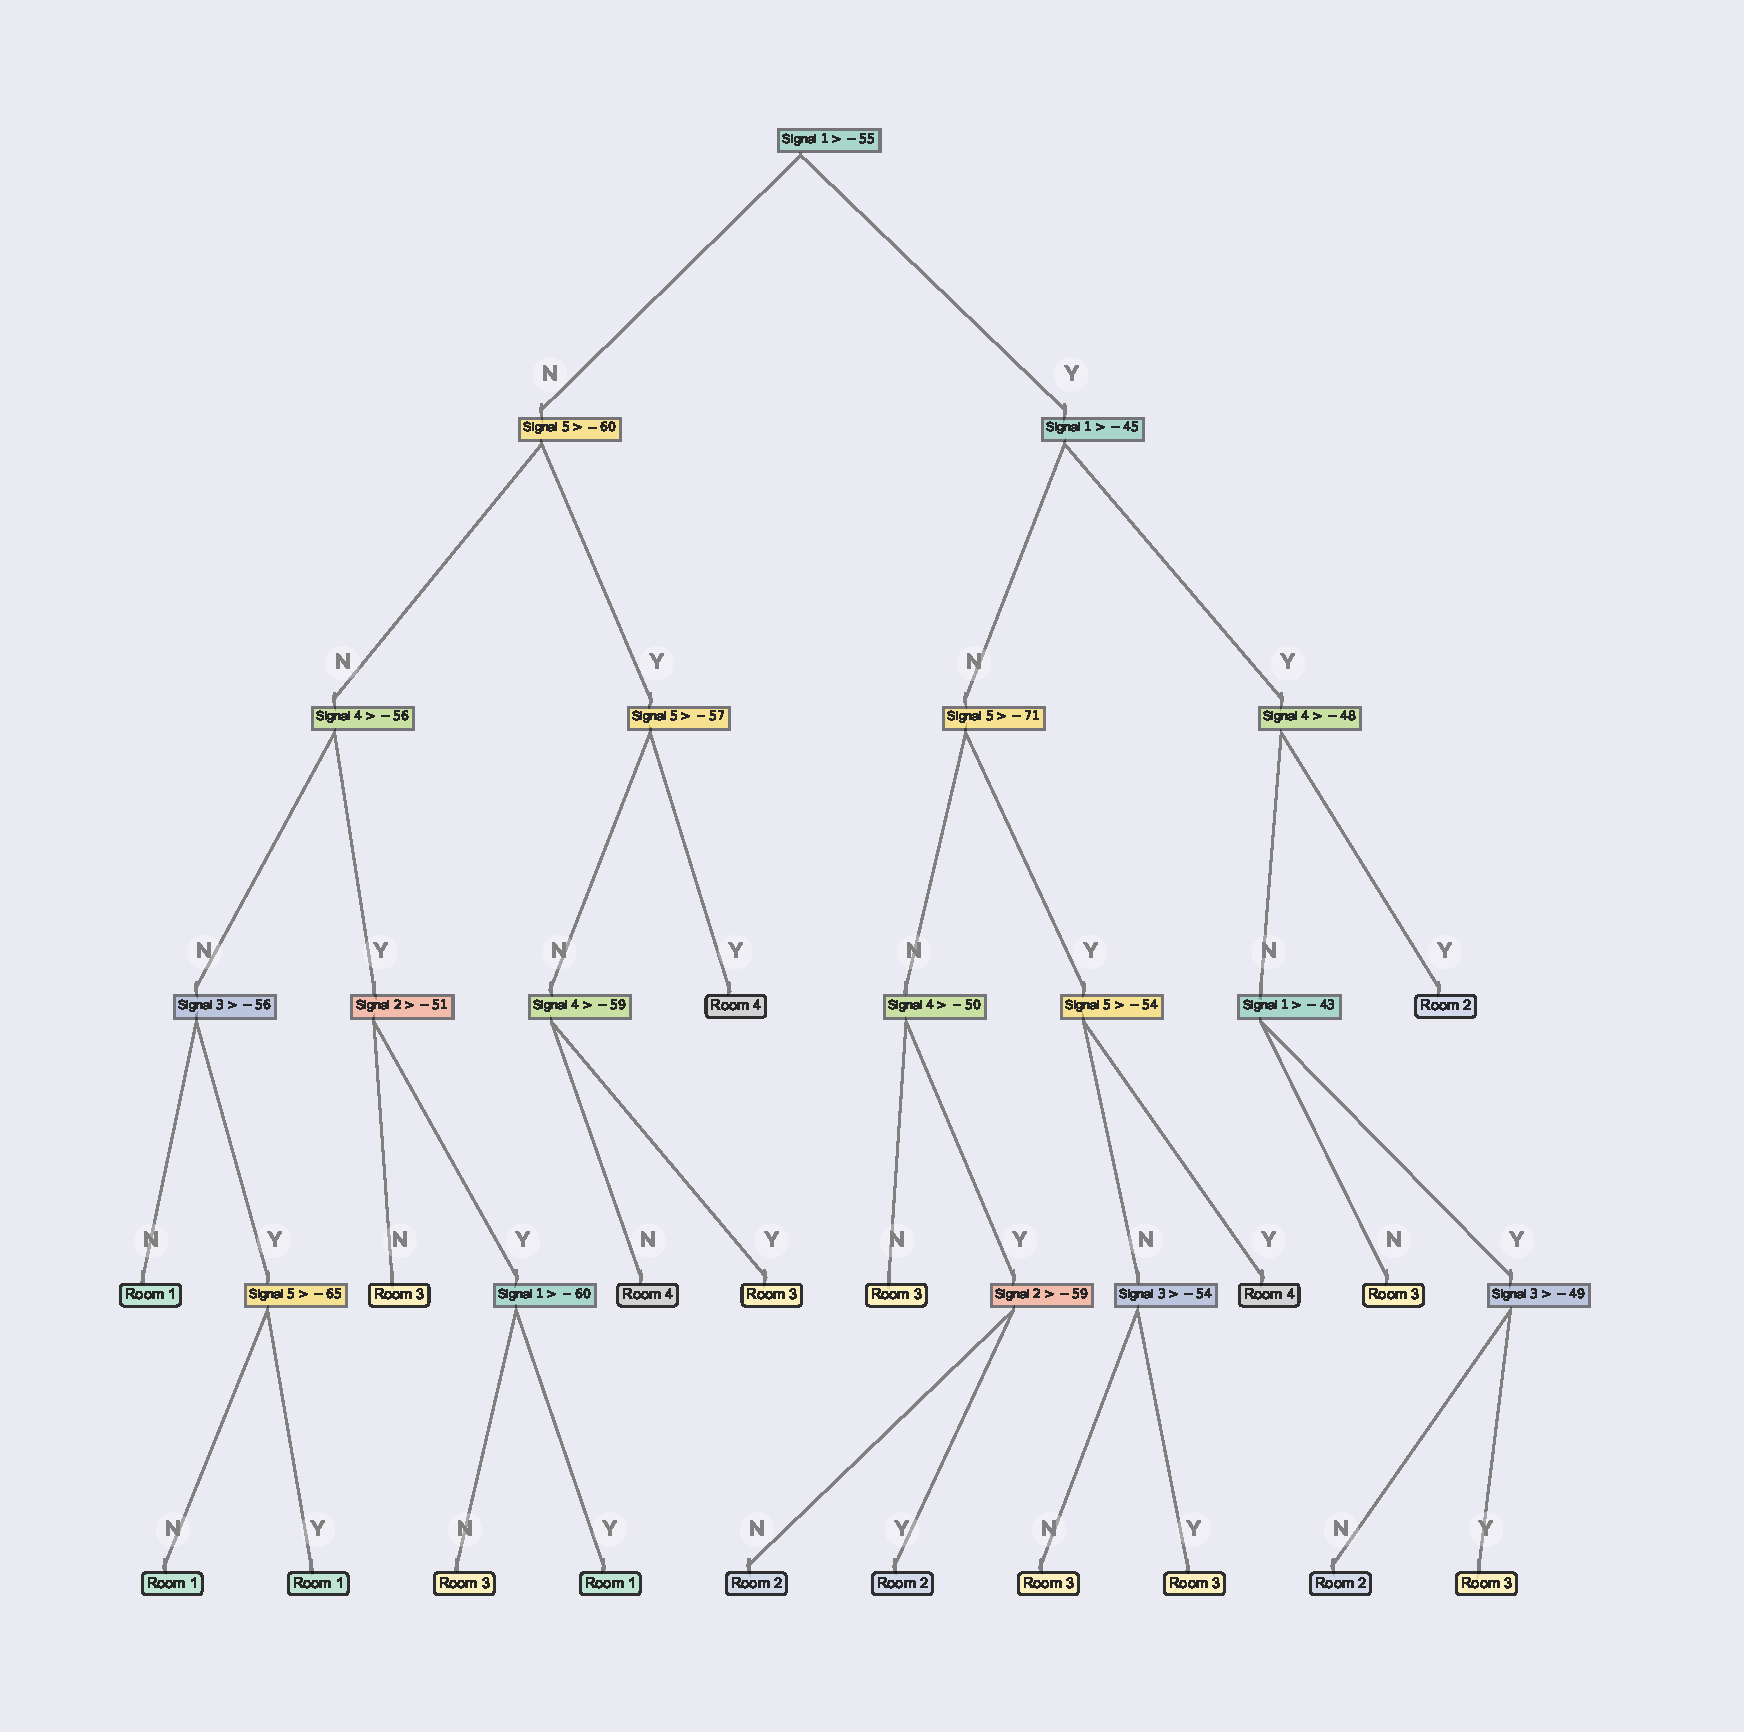
\includegraphics[width=\textwidth]{figures/clean_unpruned.pdf}
    \caption[Unpruned Tree for the Clean Dataset]{Resulting unpruned tree for the clean dataset}
    \label{fig:pruning_example_clean_unpruned}
\end{figure}

\newpage

\begin{figure}[H]
    \centering
    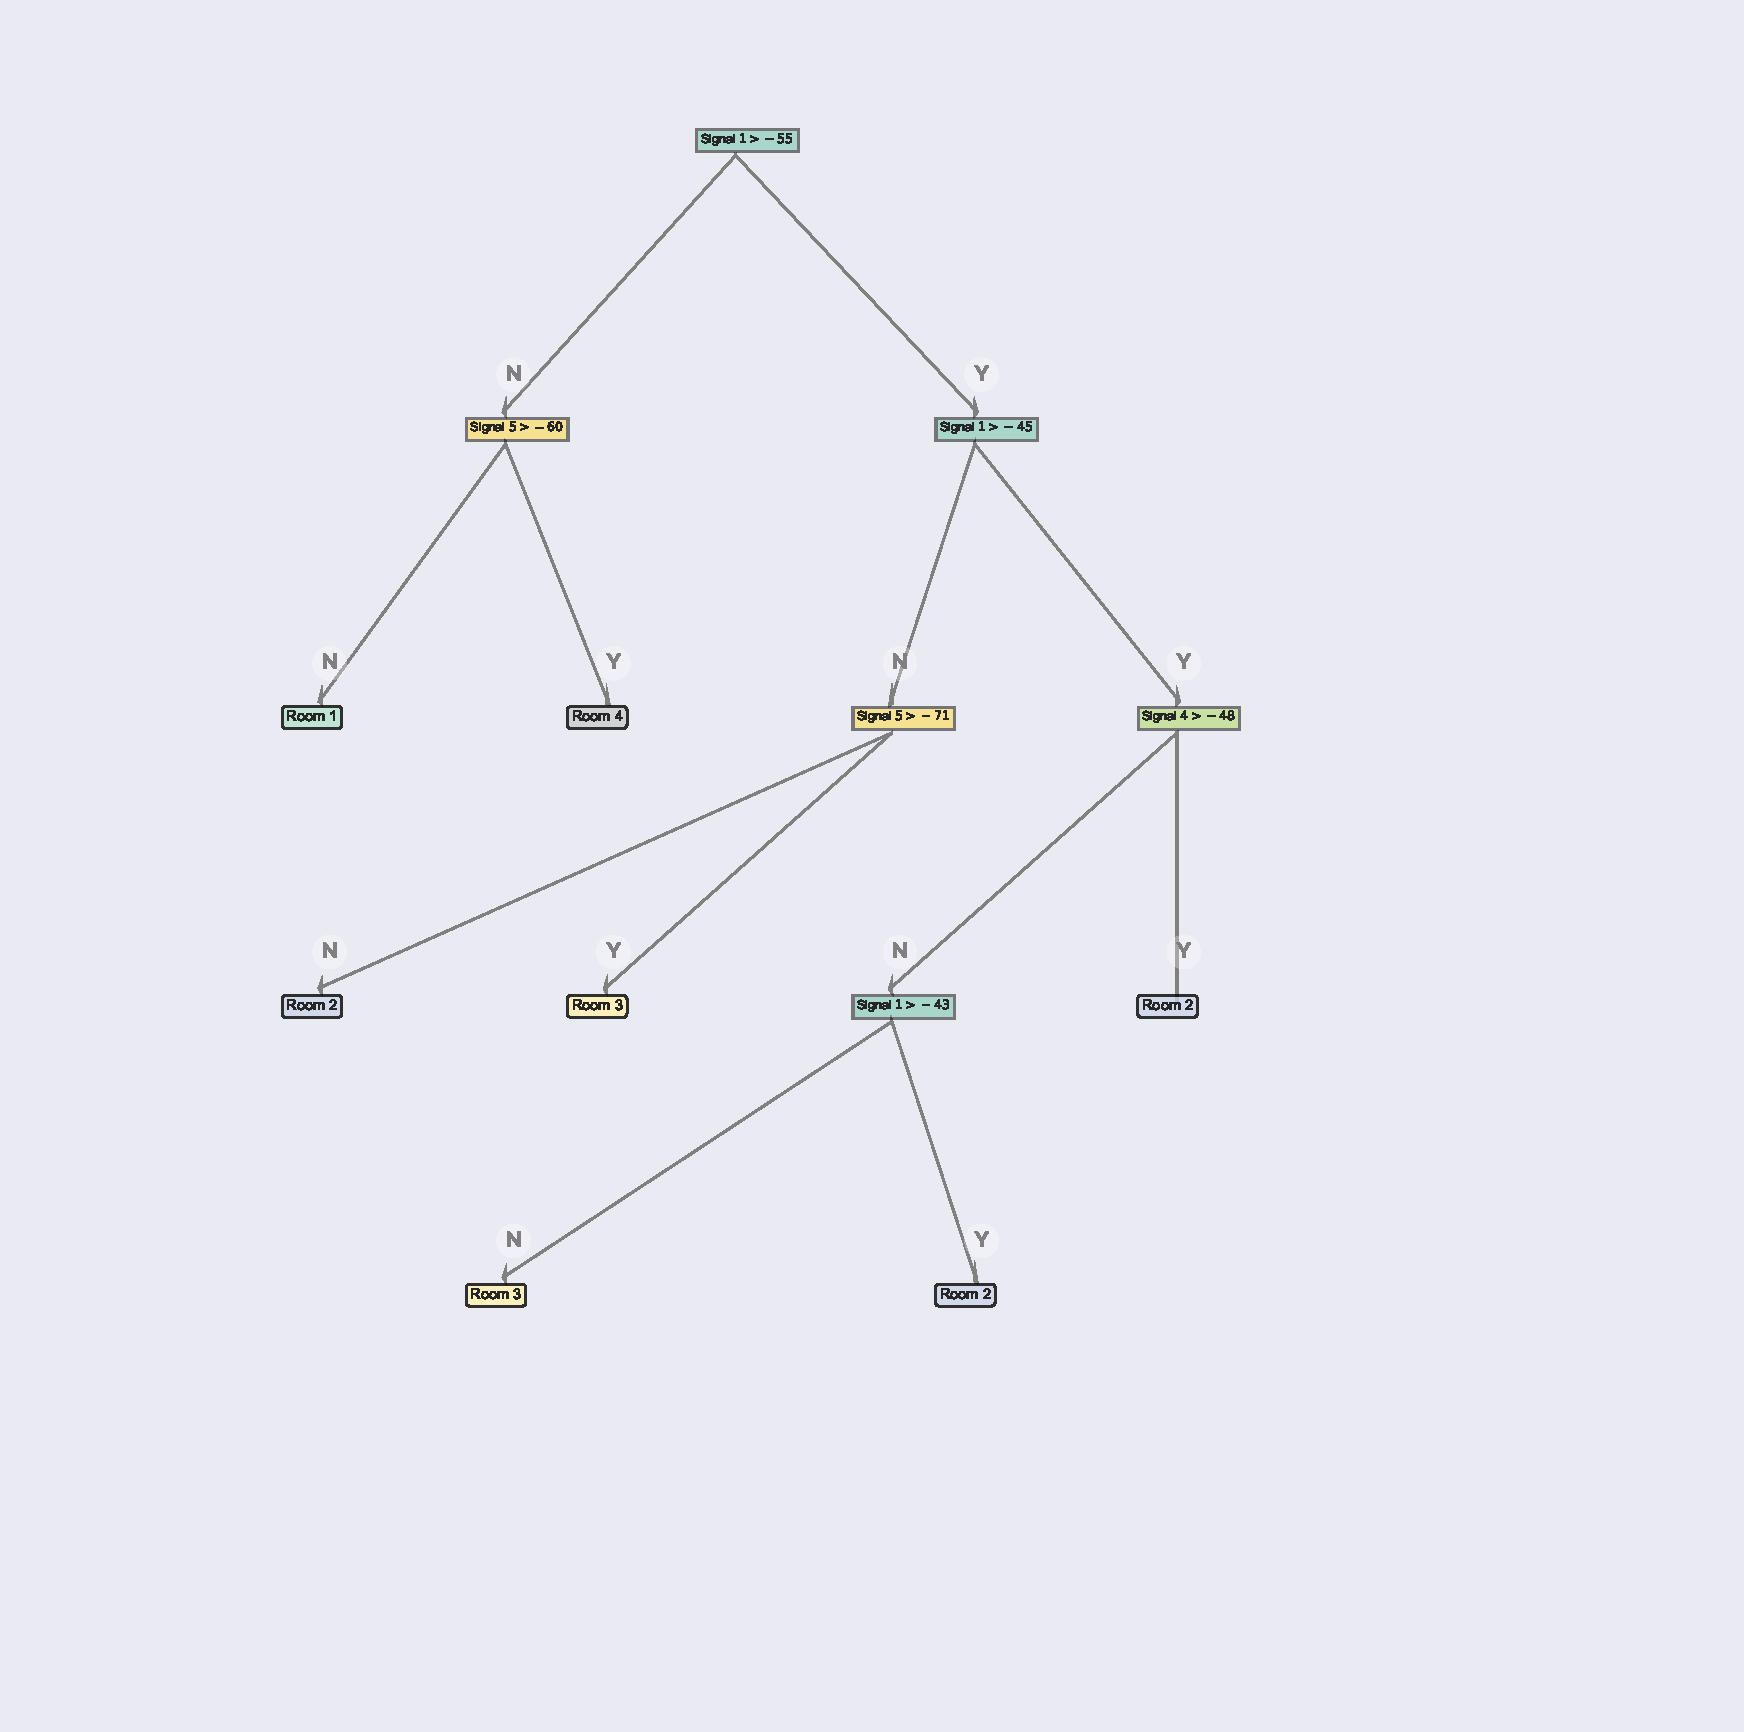
\includegraphics[width=\textwidth]{figures/clean_pruned.pdf}
    \caption[Pruned Tree for the Clean Dataset]{Resulting pruned tree for the clean dataset}
      \label{fig:pruning_example_clean_pruned}
\end{figure}
\newpage

\subsection{Noisy Dataset}
Here we demonstrate the effect of pruning on a decision tree trained on 1800 samples of the noisy data set, and pruned on the remaining 200. For the sake of clarity in the visualization, the tree depth was capped at 5.\footnote{These visualizations are automatically generated by the Visualizer class which we implemented}
\begin{figure}[H]
    \centering
    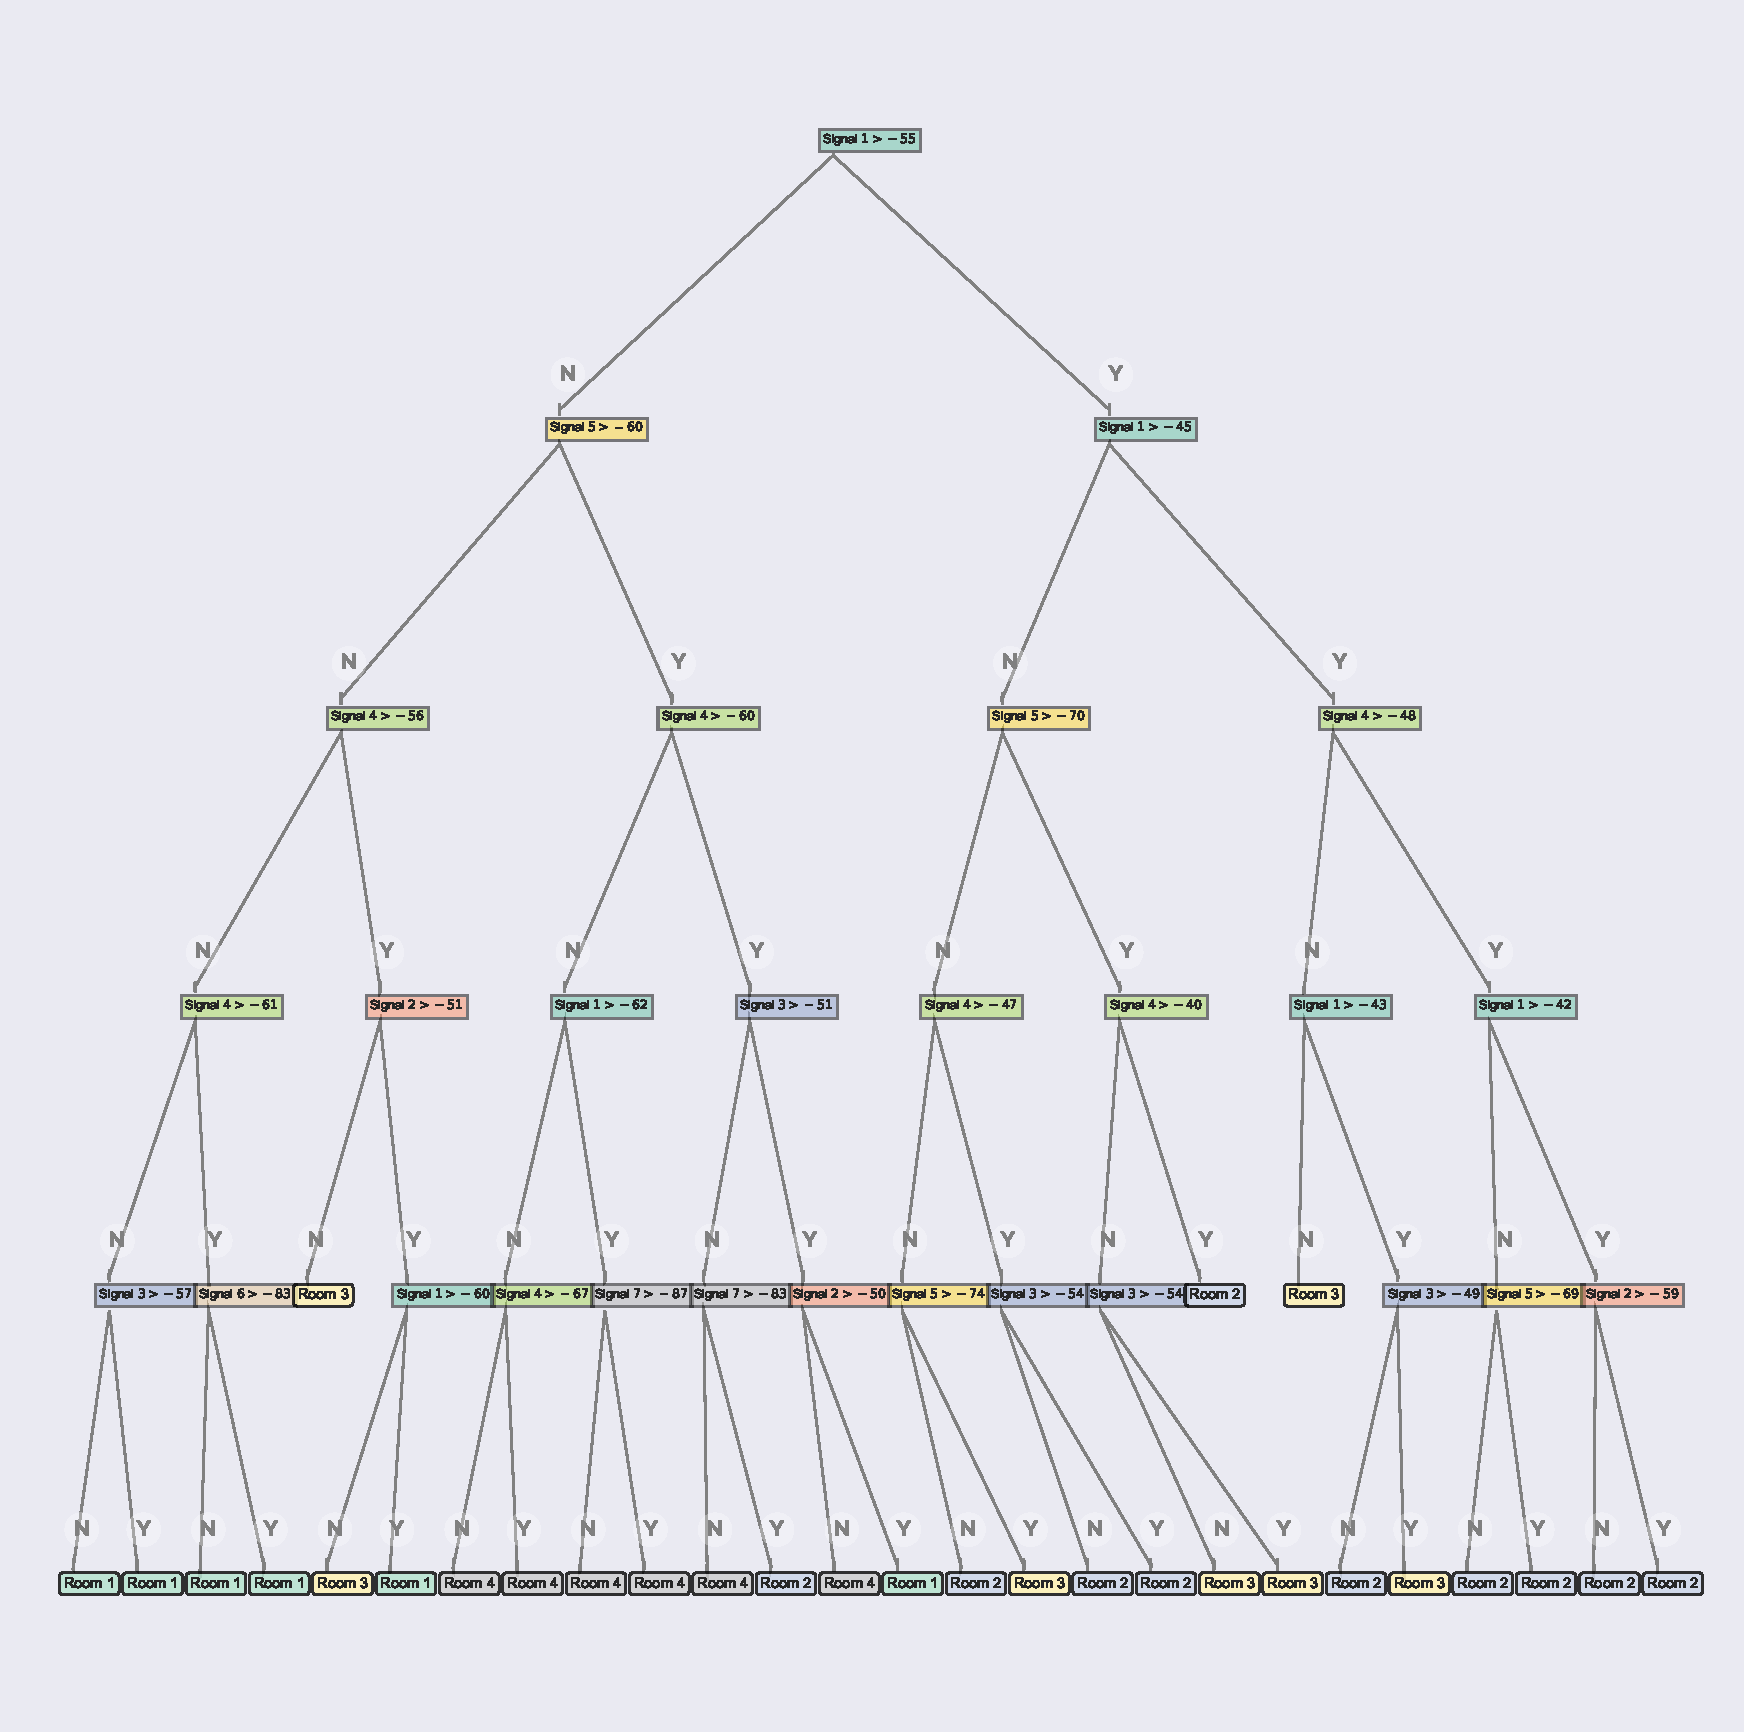
\includegraphics[width=\textwidth]{figures/noisy_unpruned.pdf}
    \caption[Unpruned Tree for the Noisy Dataset]{Resulting unpruned tree for the noisy dataset}
    \label{fig:pruning_example_noisy_unpruned}
\end{figure}

\newpage

\begin{figure}[H]
    \centering
    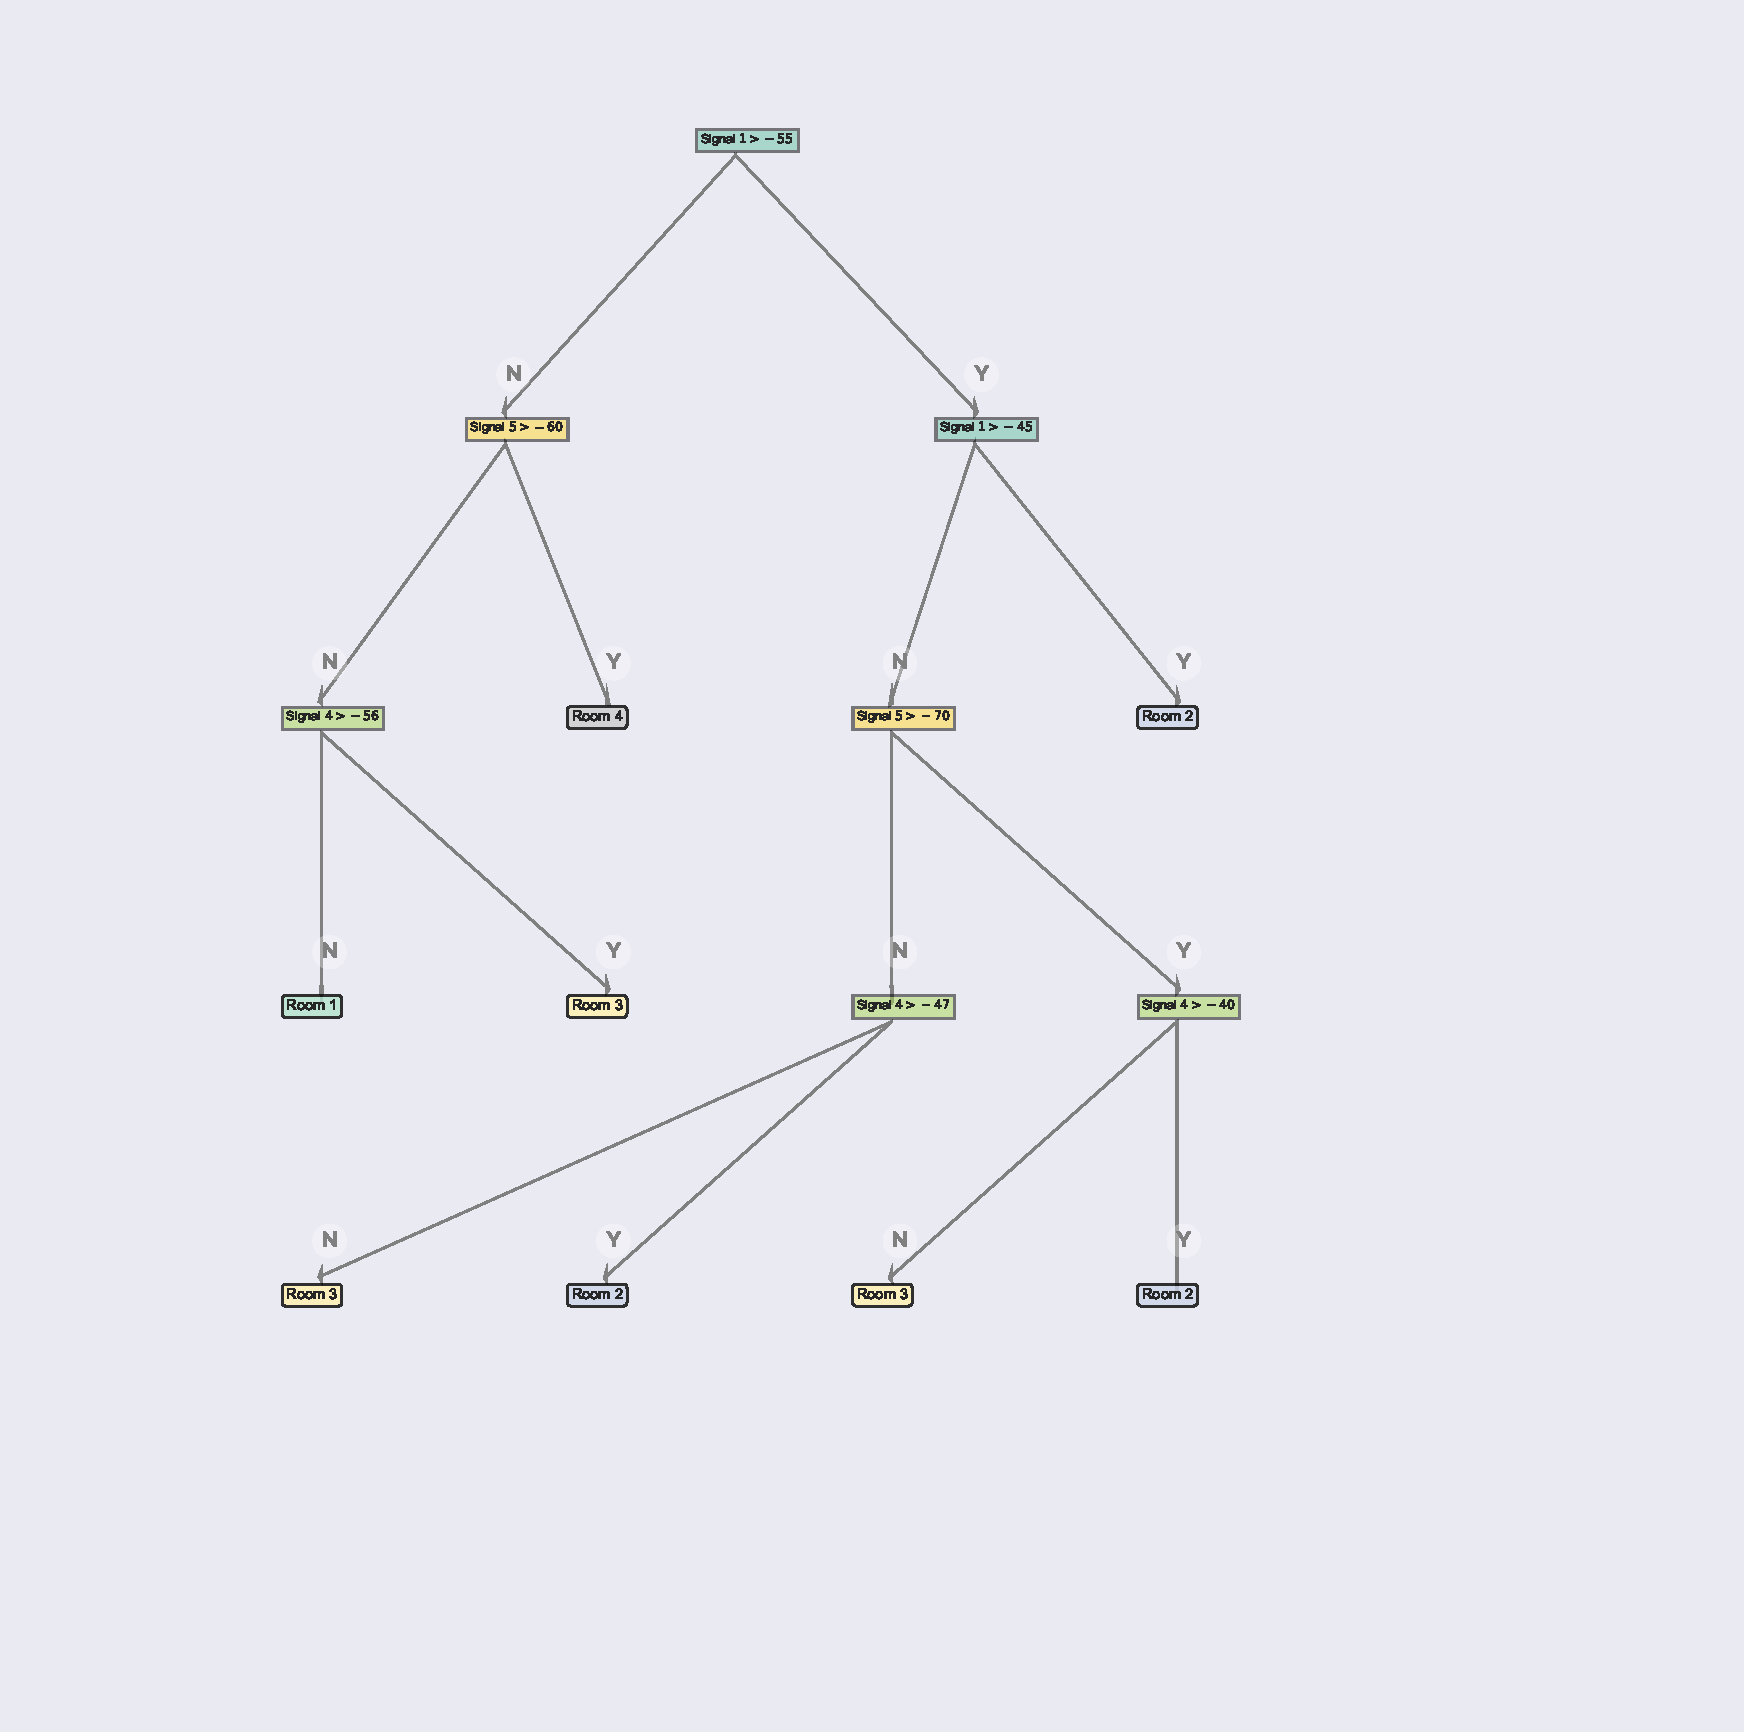
\includegraphics[width=\textwidth]{figures/noisy_pruned.pdf}
    \caption[Pruned Tree for the Noisy Dataset]{Resulting pruned tree for the noisy dataset}
      \label{fig:pruning_example_noisy_pruned}
\end{figure}
% \begin{figure}[h!]
% \centering
% 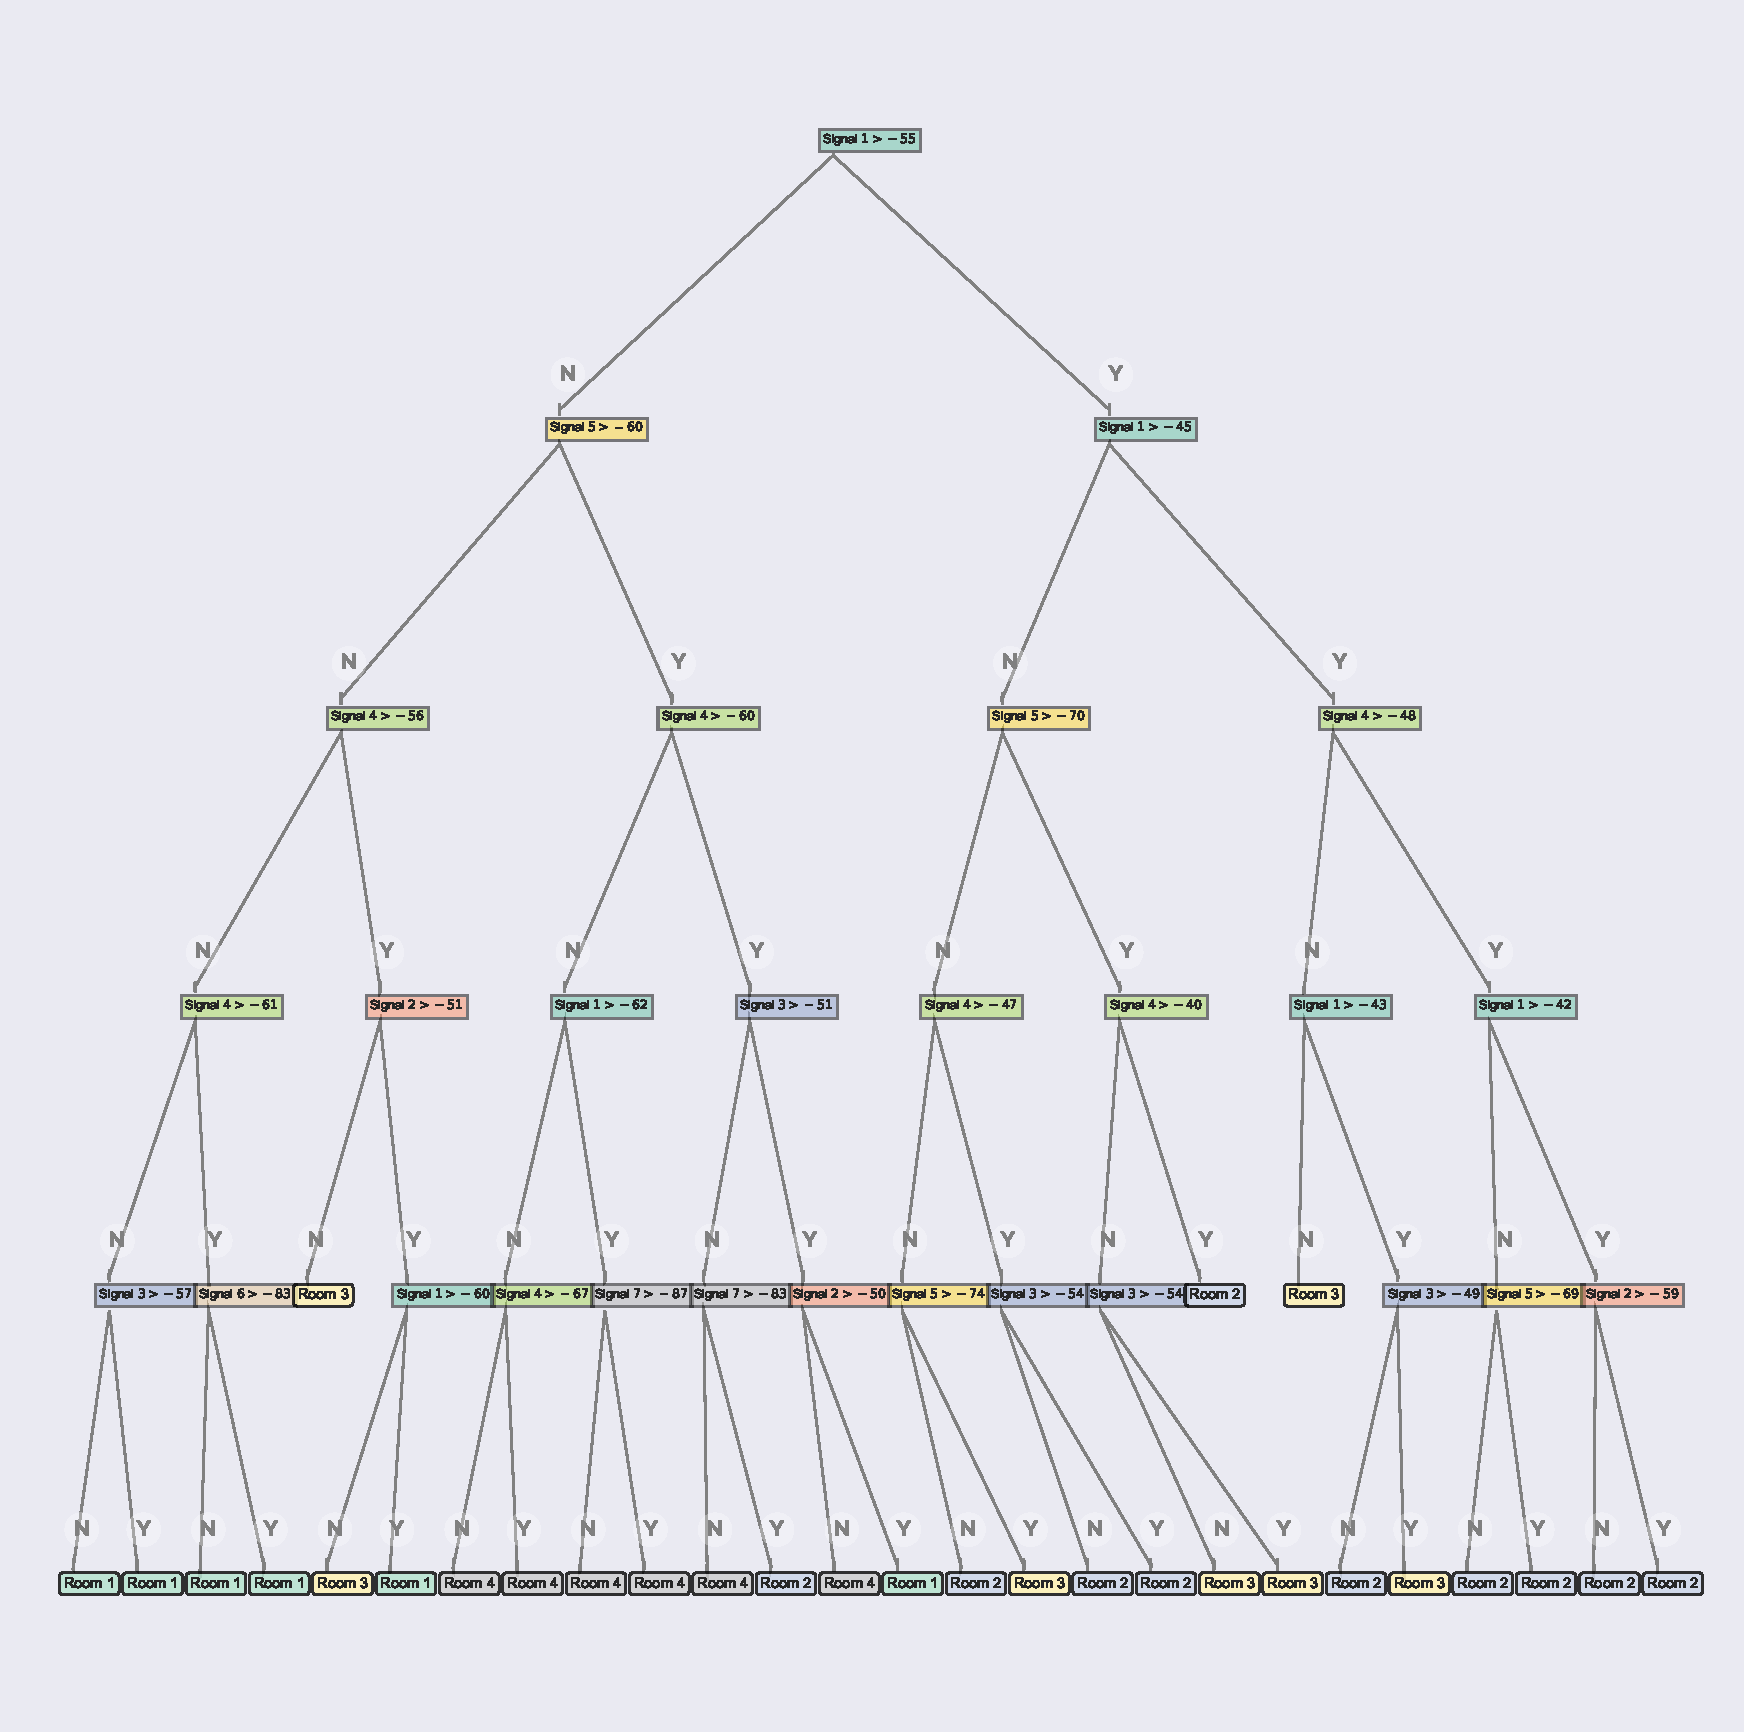
\includegraphics[width=0.65\textwidth]{figures/noisy_unpruned.pdf}
% 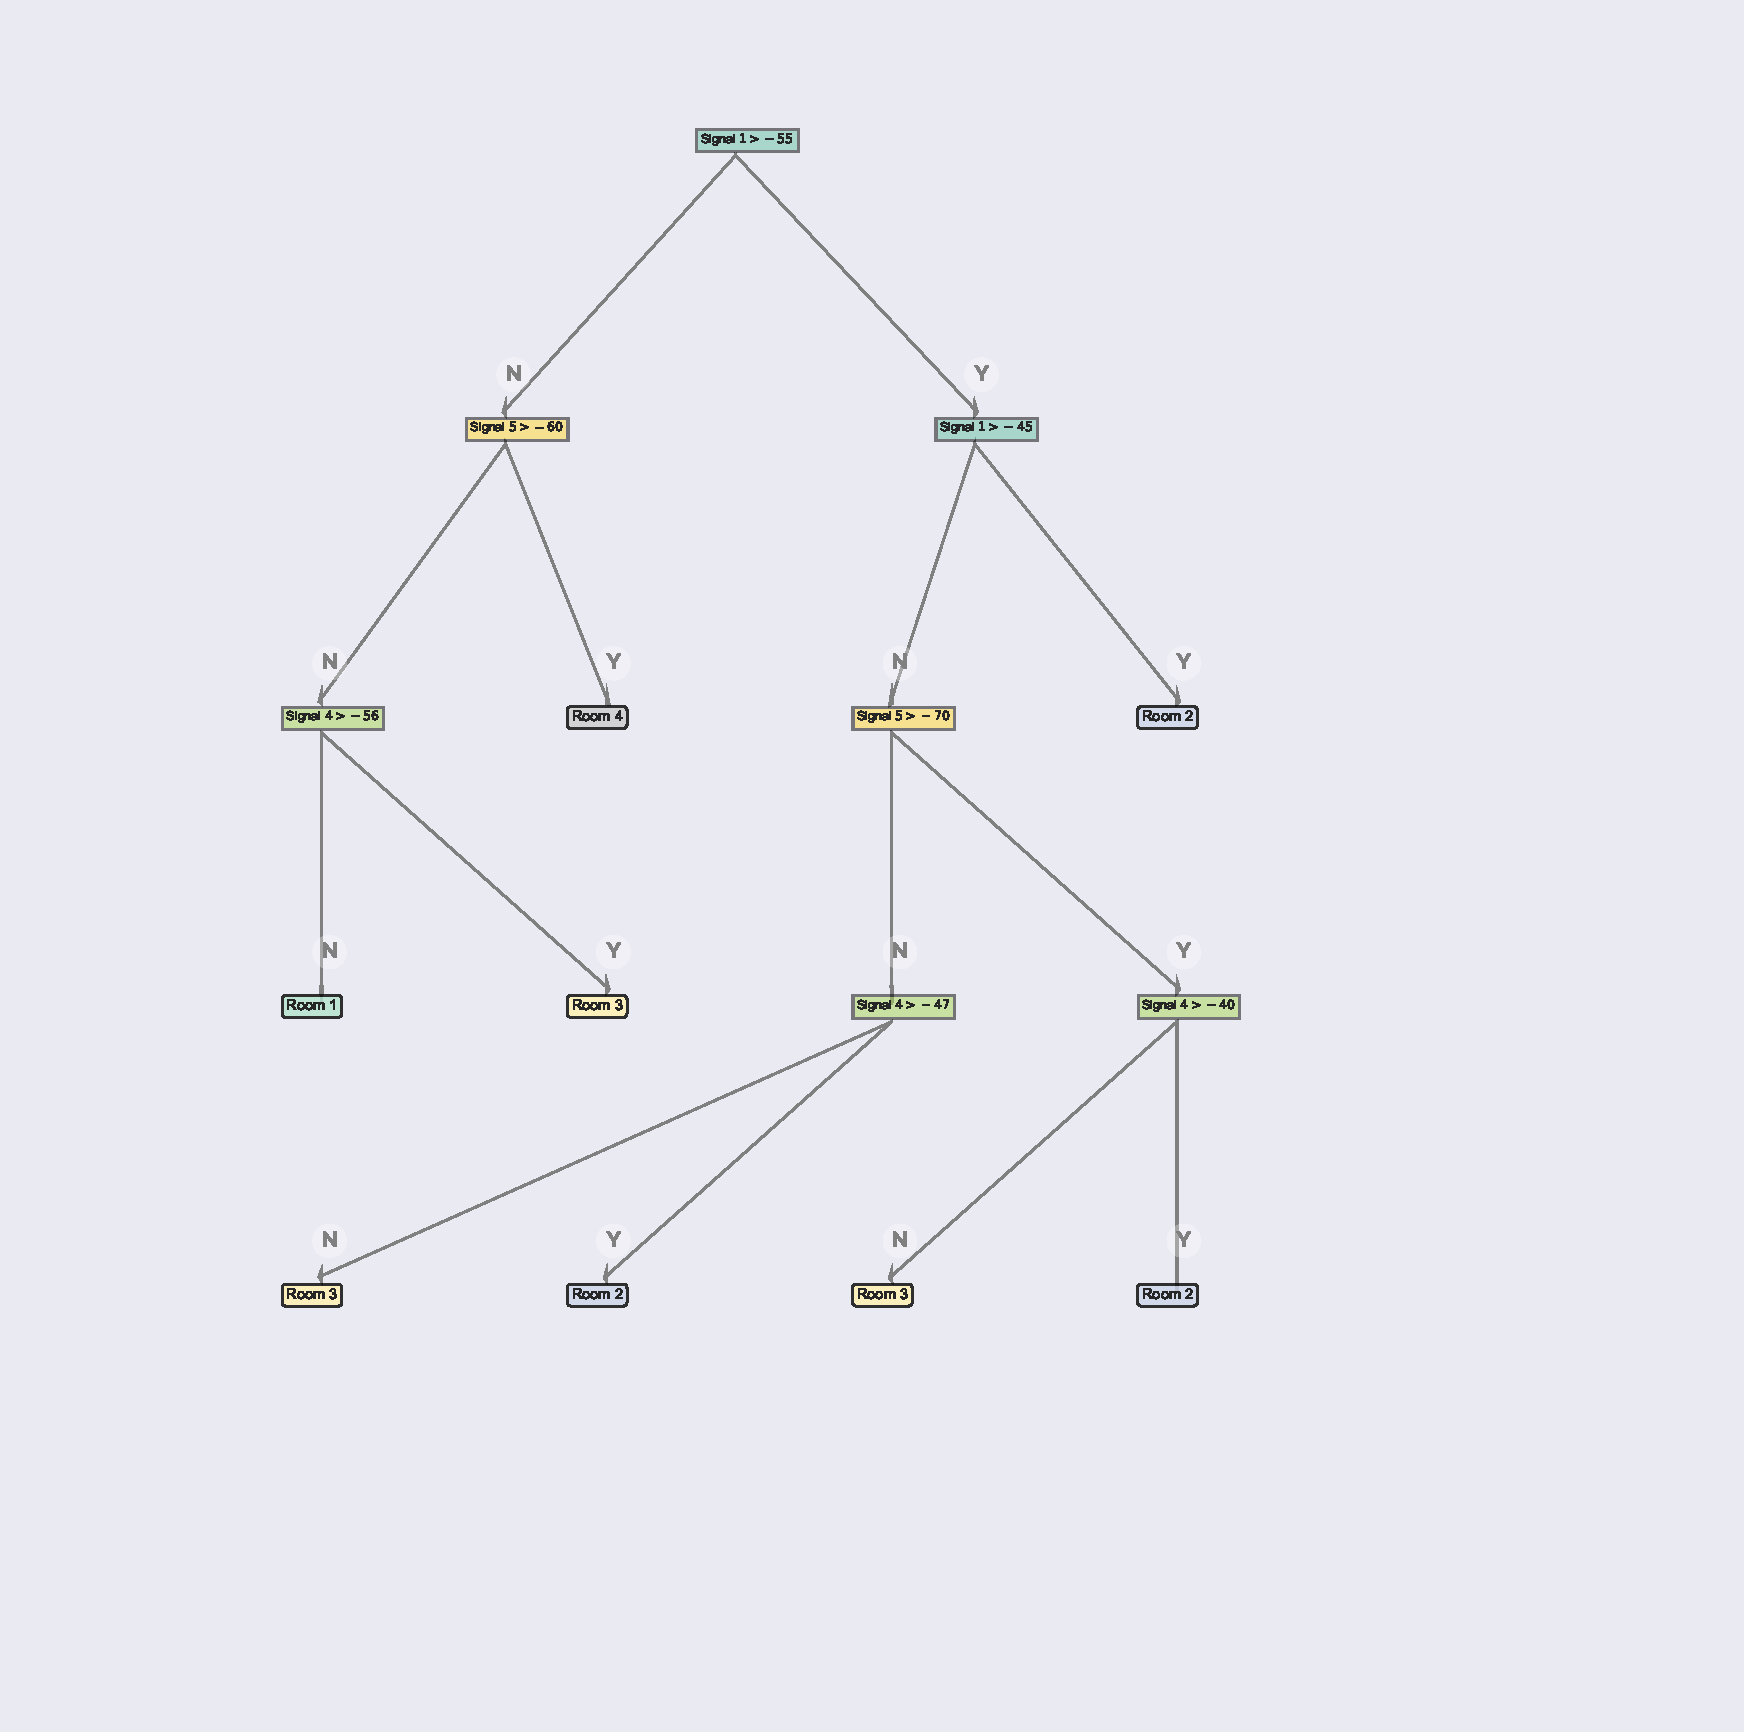
\includegraphics[width=0.65\textwidth]{figures/noisy_pruned.pdf}
% \caption{Here we demonstrate the effect of pruning on a decision tree trained on 1800 samples of the noisy data set, and pruned on the remaining 200. For the sake of clarity in the visualization, the tree depth was capped at 5.\footnote{These visualizations are automatically generated by the Visualizer class which we implemented.}}
% \
% \end{figure}
\newpage
\subsection{Entire Dataset}
Here we demonstrate the effect of pruning on a decision tree trained on 3600 samples of the total data set, and pruned on the remaining 400. The tree depth was not capped. 
\begin{figure}[H]
    \centering
    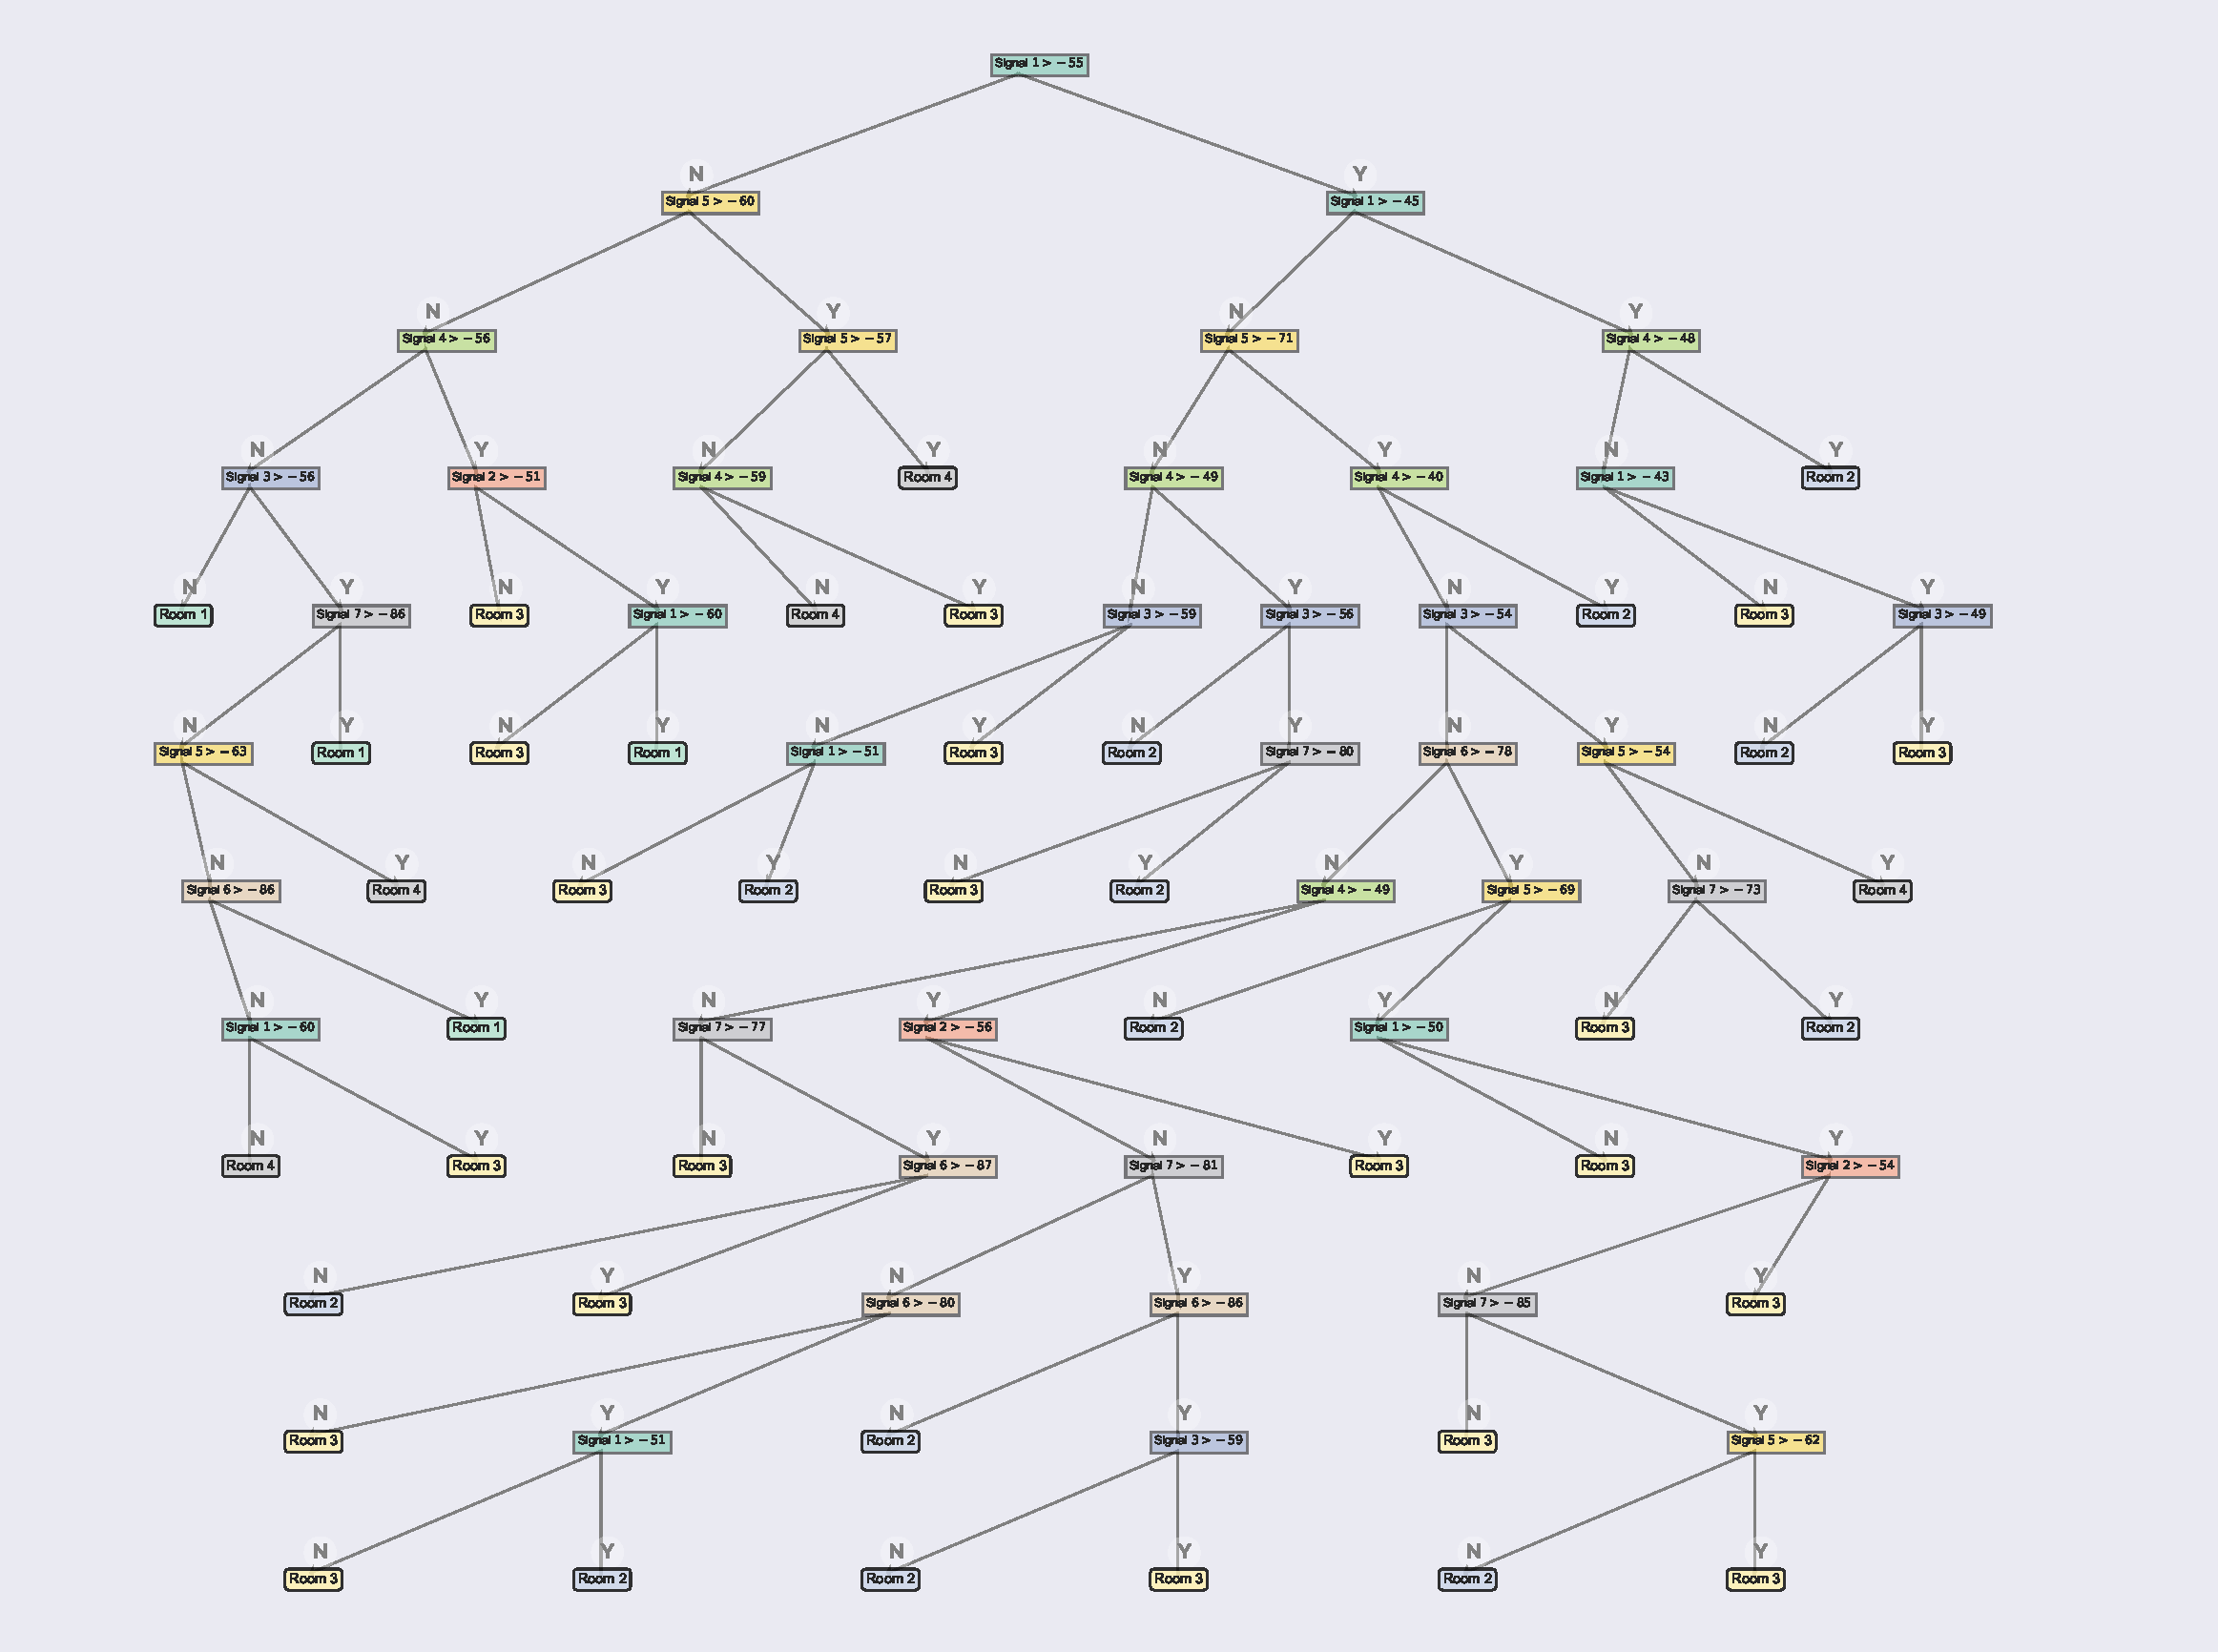
\includegraphics[width=\textwidth]{figures/total_unpruned.pdf}
    \caption[Unpruned Tree for the Entire Dataset]{Resulting unpruned tree for the entire dataset}
    \label{fig:pruning_example_total_unpruned}
\end{figure}

\newpage
\begin{figure}[H]
    \centering
    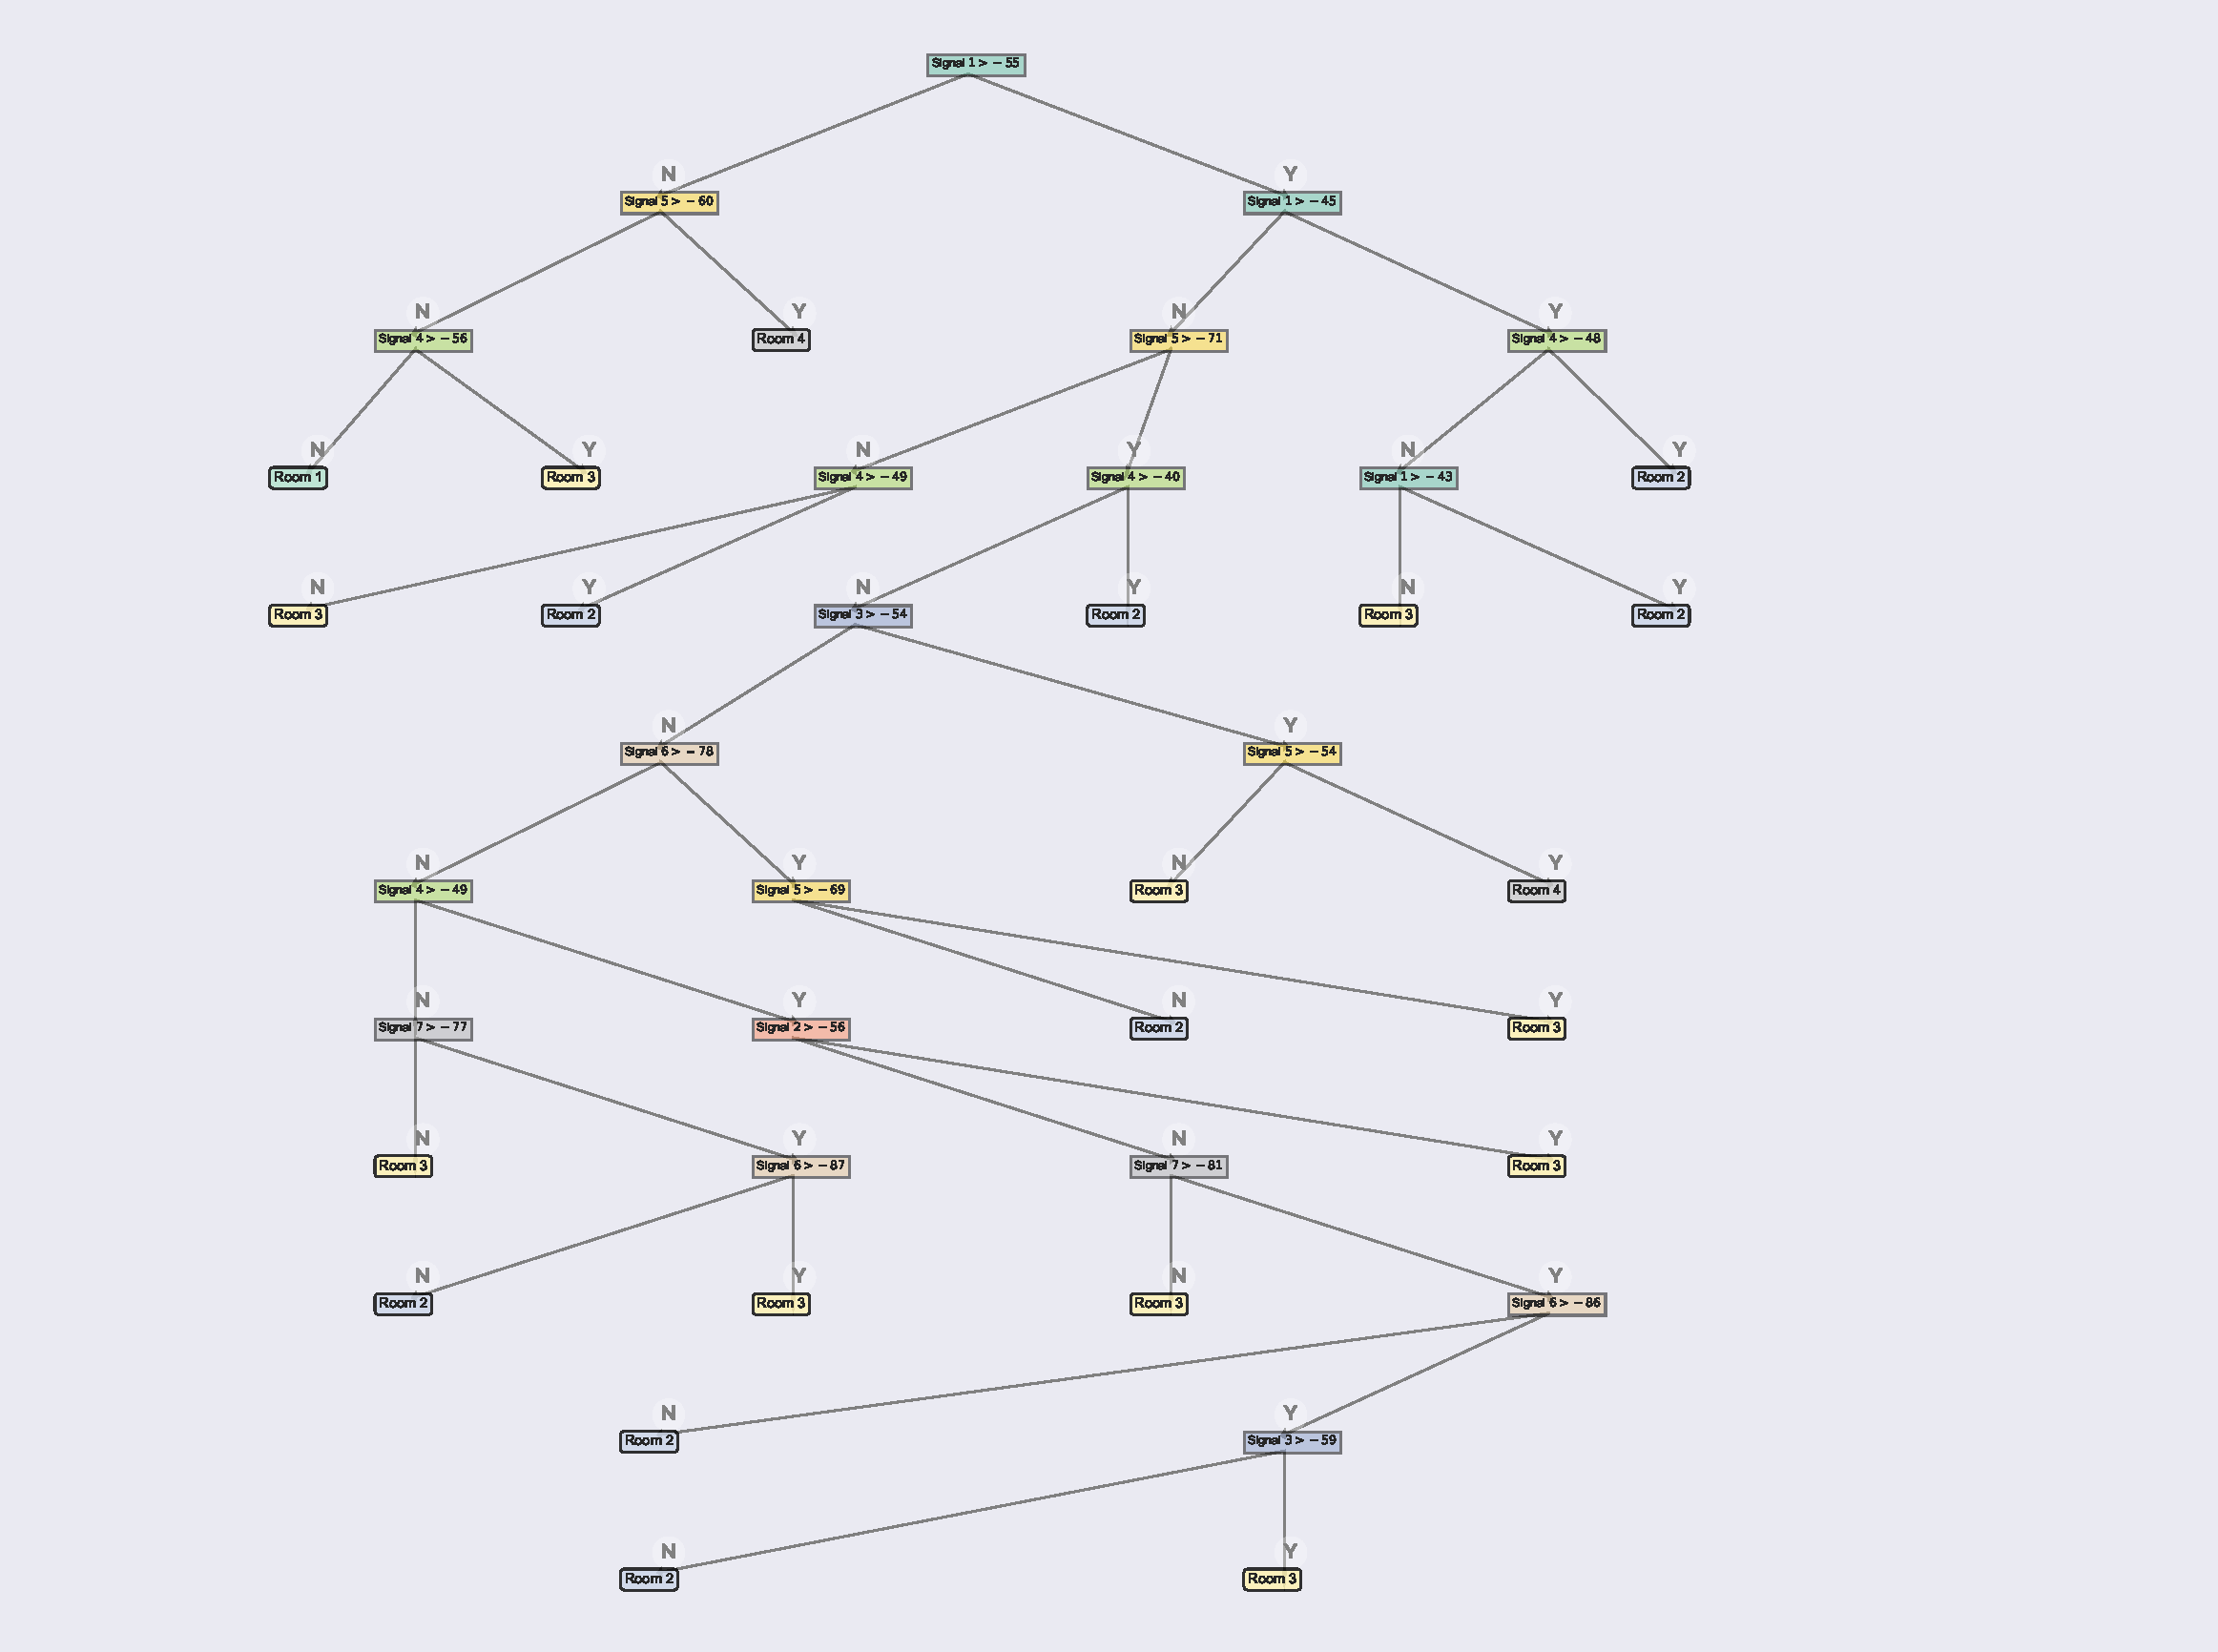
\includegraphics[width=\textwidth]{figures/total_pruned.pdf}
    \caption[Pruned Tree for the Entire Dataset]{Resulting pruned tree for the entire dataset}
      \label{fig:pruning_example_total_pruned}
\end{figure}